\documentclass[xcolor={x11names, rgb, usenames, dvipsnames}]{beamer}
% Beamer loads xcolor by default. Do not load it a second time using \usepackage

\usepackage[francais, english]{babel}
\usepackage[T1]{fontenc}
\usepackage[utf8]{inputenc}
\usepackage{pgfplots}
\pgfplotsset{compat=1.12}
\usetikzlibrary{patterns}
\usepackage{graphicx}
\usepackage{hyperref}
\usepackage{amsmath}
\usepackage{amssymb}


\setbeamertemplate{bibliography item}{[\theenumiv]}

%\usetheme{Warsaw}
% \usetheme{Boadilla}
% \usetheme{Antibes}
\usetheme{CambridgeUS}
% \usecolortheme{dolphin}
\usecolortheme{dolphin}
% \usetheme{Berlin}
% \usetheme{Madrid}
% \setbeamertemplate{footline}[frame number]


%http://tex.stackexchange.com/questions/160825/modifying-margins-for-one-slide
\newcommand\Wider[2][3em]{%
\makebox[\linewidth][c]{%
  \begin{minipage}{\dimexpr\textwidth+#1\relax}
  \raggedright#2
  \end{minipage}%
  }%
}




% http://tex.stackexchange.com/questions/116077/presentation-beamer-title-page
\makeatletter
\newcommand\titlegraphicii[1]{\def\inserttitlegraphicii{#1}}
\titlegraphicii{}
\setbeamertemplate{title page}
{
  \vbox{}
  \vspace{-2.5em}
   {\usebeamercolor[fg]{titlegraphic}\inserttitlegraphic\hfill\inserttitlegraphicii\par}
  \vskip2.5em
  \begin{centering}
    \begin{beamercolorbox}[sep=8pt,center]{institute}
      \usebeamerfont{institute}\insertinstitute
    \end{beamercolorbox}
    \begin{beamercolorbox}[sep=8pt,center]{title}
      \usebeamerfont{title}\inserttitle\par%
      \ifx\insertsubtitle\@empty%
      \else%
        \vskip0.25em%
        {\usebeamerfont{subtitle}\usebeamercolor[fg]{subtitle}\insertsubtitle\par}%
      \fi%     
    \end{beamercolorbox}%
    \vskip1em\par
    \begin{beamercolorbox}[sep=8pt,center]{date}
      \usebeamerfont{date}\insertdate
    \end{beamercolorbox}%\vskip0.5em
    \begin{beamercolorbox}[sep=8pt,center]{author}
      \usebeamerfont{author}\insertauthor
    \end{beamercolorbox}
  \end{centering}
  %\vfill
}
\makeatother

\author{Quentin Delhaye}
\title[Crypto using a Soc Platform]{Implementation of High-Level\\ Cryptographic Protocols using a SoC platform}
% \subtitle{}
\institute[ULB]{Université Libre de Bruxelles}
\date{June 24th, 2015}

\titlegraphic{
\includegraphics[width=1.5cm]{ulbnorm}}
\titlegraphicii{
\includegraphics[width=1.5cm]{logo-polytech-seul}}


%%%%%%%%%%%%%%%%%%%%%%%%
% data
%%%%%%%%%%%%%%%%%%%%%%%%
\def\temperaturedata{temperaturesOslo.txt}
\tikzstyle{maxmark} = [mark=*,mark options={color=red,scale=15}]
\tikzstyle{minmark} = [mark=*,mark options={color=blue,scale=15}]

% Lists
% \def\labelitemi{$\blacktriangleright$}

% \AtBeginSection[]
% {
%   \begin{frame}
%   \frametitle{Contents}
%   \tableofcontents[currentsection]
%   \end{frame}
% }


\begin{document}

\begin{frame}[plain, noframenumbering]
\titlepage
\end{frame}

\begin{frame}
	\frametitle{Contents}
	\tableofcontents[hideallsubsections]
	% \tableofcontents
\end{frame}


\section{Context}

\begin{frame}
\begin{itemize}
	\item Internet of things
	\item More connections, less power, same security
	% And this is essential to understand the complexity of the problem.
	% How to ensure the same security level with less computing power at hand?
	\item Work done with Barco Silex
\end{itemize}
\end{frame}

\subsection{Objectives}
\begin{frame}
\frametitle{Objectives}
\begin{itemize}
	\item Real life use cases.
	\item Decrease CPU load.
	\item Improve performance.
\end{itemize}
\end{frame}







\section{Cryptographic protocols}
% \begin{frame}
% \frametitle{Contents}
% \tableofcontents[currentsection]
% \end{frame}

\begin{frame}
\frametitle{Cryptographic protocols}
\begin{description}
	\item[VPN]~\\
		\begin{itemize}
			\item TLS
			\item IPsec
		\end{itemize}
	\item[Schemes]~\\
		\begin{itemize}
			\item AES
			\item SHA-2
			\item Diffie-Hellman
			\item RSA
		\end{itemize}
\end{description}
\end{frame}



\section{Platform}
\begin{frame}
\frametitle{Contents}
\tableofcontents[%
	currentsection,
	sectionstyle=show/shaded,%Show the current section, shade the others
	subsectionstyle=show/show/hide,%Show the current subsection, show the other subsections of the same section, hide the other other subsections.
	]
\end{frame}


\subsection{Hardware}
\begin{frame}
\frametitle{SoCrates}
	\begin{figure}
	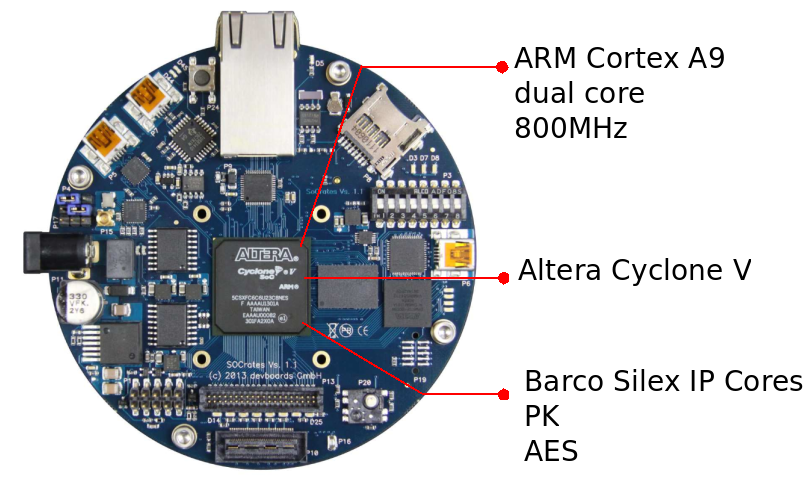
\includegraphics[height=6cm]{socrates-annotated.png}
	\end{figure}
	% Low-end FPGA. It's an affordable board that has been used as a proof-of-concept implementation.
	% It can only get better with more expensive and more recent technologies.
	% However, the Cortex A9 is nice already, so the software is already close to its full potential.
\end{frame}


\subsection{Operating System}
\begin{frame}
\frametitle{Linux structure}
	\begin{center}
	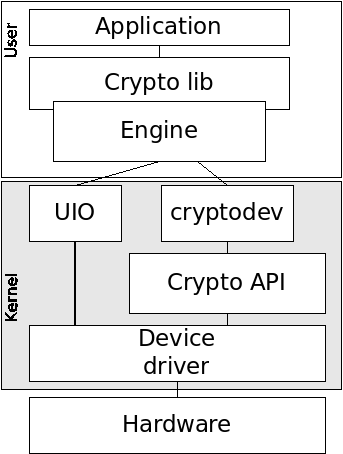
\includegraphics[height=7cm]{os-path-generic.png}
	\end{center}
\end{frame}


\begin{frame}
\frametitle{Linux structure (Cont'd)}
	\begin{center}
	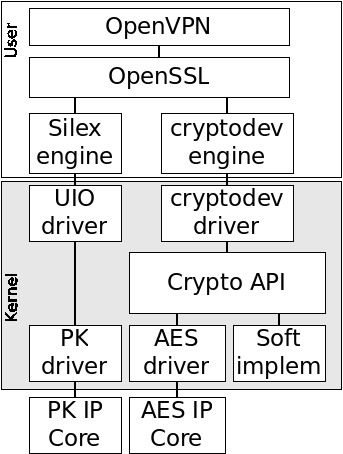
\includegraphics[height=7cm]{os-path-specific.png}
	\end{center}
\end{frame}





\section{Implementation}
\begin{frame}
\frametitle{Contents}
\tableofcontents[%
	currentsection,
	sectionstyle=show/shaded,
	subsectionstyle=show/show/hide,
	]
\end{frame}

\subsection{OpenVPN}
\begin{frame}
\frametitle{OpenVPN}
	\begin{figure}
	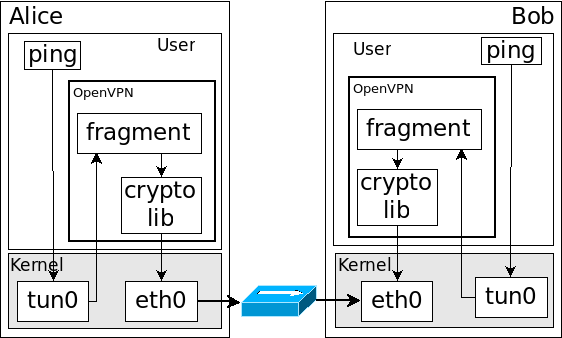
\includegraphics[height=6cm]{openvpn-transfer.png}
	\end{figure}
\end{frame}

\subsection{IPsec}
\begin{frame}
\frametitle{IPsec}
	\begin{figure}
	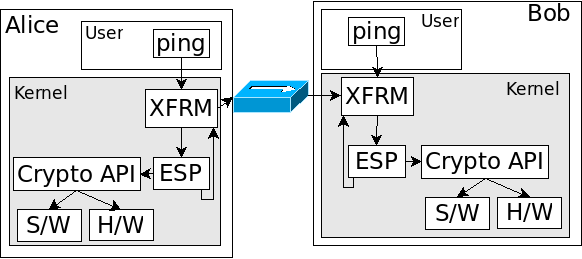
\includegraphics[height=5cm]{ipsec-transfer.png}
	\end{figure}
\end{frame}




\section{Results}
\begin{frame}
\frametitle{Contents}
\tableofcontents[%
	currentsection,
	sectionstyle=show/shaded,
	subsectionstyle=show/show/hide,
	]
\end{frame}


\subsection{TLS connections}

\begin{frame}
\frametitle{TLS connections -- Context}
\begin{center}
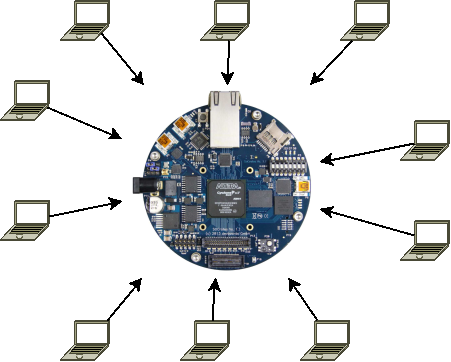
\includegraphics[height=3cm]{tls-bench.png}
\end{center}
\begin{itemize}
	\item 1 server, 10 clients
	\item 1-second connections
	\item RSA-1024/2048/4096
	\item OpenVPN
\end{itemize}
\end{frame}

\begin{frame}
\frametitle{TLS connections -- OpenVPN}
\Wider[1em]{%
	\begin{minipage}[c]{.48\linewidth}
		\begin{tikzpicture}
		%%%%%%%%%%%%%%%%%%%%%%%%
% throughput
%%%%%%%%%%%%%%%%%%%%%%%%
\begin{axis}[
        % title = {FTP transfer inside an IPSec tunnel},
        width  = \textwidth,
        height = 0.65\paperheight,
        major x tick style = transparent,
        xbar=2pt,
        bar width=8pt,
        % enlarge x limits={abs=1},
        xmajorgrids = true,
        xlabel = {Connections per minute},
        ylabel = {},
        ylabel near ticks,
        yticklabel pos=right,
        xmin=0, xmax=600,
        xtick={0,100,200,300,400,500},
        symbolic y coords={RSA-1024, RSA-2048, RSA-4096},
        ytick = data,
        scaled x ticks = false,%Disable the *10^4 exponent applied to all y axis markings.
        legend style={at={(1.3,-0.1)}, anchor=north,legend columns=1},
        % enlarge x limits=0.1,
    ]

\addplot[style={black,fill=ForestGreen,mark=none}, nodes near coords={\pgfmathfloatifflags{\pgfplotspointmeta}{0}{}{\pgfmathprintnumber{\pgfplotspointmeta}}}]
    coordinates {
        (445.4,RSA-1024)
        (155.6,RSA-2048)
        (19.6,RSA-4096)
    };
    \label{soft-tp}

\addplot[style={black,fill=BrickRed,mark=none}, nodes near coords={\pgfmathfloatifflags{\pgfplotspointmeta}{0}{}{\pgfmathprintnumber{\pgfplotspointmeta}}}]
    coordinates {
        (509.3,RSA-1024)
        (420.9,RSA-2048)
        (115.5,RSA-4096)
    };
    \label{ba411e-tp}
\legend{\small software, H/W}
\end{axis}
		\end{tikzpicture}
	\end{minipage} \hfill
	\begin{minipage}[c]{.44\linewidth}
		\begin{tikzpicture}
		%%%%%%%%%%%%%%%%%%%%%%%%
% throughput
%%%%%%%%%%%%%%%%%%%%%%%%
\begin{axis}[
        % title = {FTP transfer inside an IPSec tunnel},
        width  = \textwidth,
        height = 0.65\paperheight,
        major x tick style = transparent,
        xbar=2pt,
        bar width=8pt,
        % enlarge x limits={abs=1},
        xmajorgrids = true,
        xlabel = {CPU usage},
        ylabel = {},
        % ylabel near ticks,
        % yticklabel pos=right,
        xmin=0, xmax=115,
        xtick={50, 100},
        symbolic y coords={RSA-1024, RSA-2048, RSA-4096},
        ytick = data,
        ymajorticks=false,
        scaled x ticks = false,%Disable the *10^4 exponent applied to all y axis markings.
        legend style={at={(0.5,-0.15)}, anchor=north,legend columns=4},
        % enlarge x limits=0.1,
    ]

\addplot[style={black,fill=LimeGreen,postaction={pattern=north east lines},mark=none}, nodes near coords={\pgfmathfloatifflags{\pgfplotspointmeta}{0}{}{\pgfmathprintnumber{\pgfplotspointmeta}}}]
    coordinates {
        (40.32,RSA-1024)
        (92.14,RSA-2048)
        (81.97,RSA-4096)
    };
    \label{software}

\addplot[style={black,fill=RedOrange,postaction={pattern=north east lines},mark=none}, nodes near coords={\pgfmathfloatifflags{\pgfplotspointmeta}{0}{}{\pgfmathprintnumber{\pgfplotspointmeta}}}]
    coordinates {
        (13.29,RSA-1024)
        (4.82,RSA-2048)
        (4.78,RSA-4096)
    };
    \label{ba414e}
% \legend{software, ba411e, out-of-tunnel, inside tunnel}
\end{axis}
		\end{tikzpicture}
		\vspace{0.5cm}
	\end{minipage}
}
\end{frame}


\subsection{File transfer}

\begin{frame}
\frametitle{File transfer -- Context}
\begin{center}
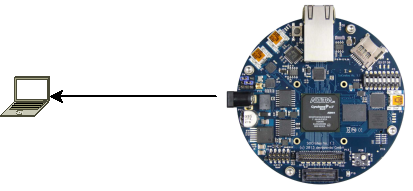
\includegraphics[height=3cm]{ftp-bench.png}
\end{center}
\begin{itemize}
	\item 128MB file
	\item AES-256-CBC/SHA-256
	\item OpenVPN/IPsec
\end{itemize}
\end{frame}

\begin{frame}
\frametitle{File transfer -- OpenVPN}
\Wider[1em]{%
	\begin{minipage}[c]{.48\linewidth}
		\begin{tikzpicture}
		%%%%%%%%%%%%%%%%%%%%%%%%
% throughput
%%%%%%%%%%%%%%%%%%%%%%%%
\begin{axis}[
        % title = {FTP transfer inside an IPSec tunnel},
        width  = \textwidth,
        height = 0.75\paperheight,
        major x tick style = transparent,
        xbar=2pt,
        bar width=8pt,
        % enlarge x limits={abs=1},
        xmajorgrids = true,
        xlabel = {Throughput [MB/s]},
        ylabel = {},
        ylabel near ticks,
        yticklabel pos=right,
        xmin=0, xmax=15,
        symbolic y coords={cipher null, aes:none, aes:sha},
        ytick = data,
        scaled x ticks = false,%Disable the *10^4 exponent applied to all y axis markings.
        legend style={at={(1.3,-0.1)}, anchor=north,legend columns=2},
        % enlarge x limits=0.1,
    ]

\addplot[style={black,fill=ForestGreen,mark=none}, nodes near coords={\pgfmathfloatifflags{\pgfplotspointmeta}{0}{}{\pgfmathprintnumber{\pgfplotspointmeta}}}]
    coordinates {
        (0,cipher null)
        (4.78,aes:none)
        (3.87,aes:sha)
    };
    \label{software}

\addplot[style={black,fill=black,mark=none}, nodes near coords={\pgfmathfloatifflags{\pgfplotspointmeta}{0}{}{\pgfmathprintnumber{\pgfplotspointmeta}}}]
    coordinates {
        (11.39,cipher null)
        (0,aes:none)
        (0,aes:sha)
    };
    \label{out-of-tunnel}%"tp" for "throughput"

\addplot[style={black,fill=BrickRed,mark=none}, nodes near coords={\pgfmathfloatifflags{\pgfplotspointmeta}{0}{}{\pgfmathprintnumber{\pgfplotspointmeta}}}]
    coordinates {
        (0,cipher null)
        (3.35,aes:none)
        (2.84,aes:sha)
    };
    \label{ba411e}

\addplot[style={black,fill=MidnightBlue,mark=none}, nodes near coords={\pgfmathfloatifflags{\pgfplotspointmeta}{0}{}{\pgfmathprintnumber{\pgfplotspointmeta}}}]
    coordinates {
        (5.18,cipher null)
        (0,aes:none)
        (0,aes:sha)
    };
    \label{inside tunnel}
\legend{\small software, raw, ba411e, OpenVPN}
\end{axis}
		\end{tikzpicture}
	\end{minipage} \hfill
	\begin{minipage}[c]{.44\linewidth}
		\begin{tikzpicture}
		%%%%%%%%%%%%%%%%%%%%%%%%
% throughput
%%%%%%%%%%%%%%%%%%%%%%%%
\begin{axis}[
        % title = {FTP transfer inside an IPSec tunnel},
        width  = \textwidth,
        height = 0.75\paperheight,
        major x tick style = transparent,
        xbar=2pt,
        bar width=8pt,
        % enlarge x limits={abs=1},
        xmajorgrids = true,
        xlabel = {CPU usage},
        ylabel = {},
        % ylabel near ticks,
        % yticklabel pos=right,
        xmin=0, xmax=115,
        xtick={50, 100},
        symbolic y coords={cipher null, aes:none, aes:sha},
        ytick = data,
        ymajorticks=false,
        scaled x ticks = false,%Disable the *10^4 exponent applied to all y axis markings.
        legend style={at={(0.5,-0.15)}, anchor=north,legend columns=4},
        % enlarge x limits=0.1,
    ]

\addplot[style={black,fill=LimeGreen,postaction={pattern=north east lines},mark=none}, nodes near coords={\pgfmathfloatifflags{\pgfplotspointmeta}{0}{}{\pgfmathprintnumber{\pgfplotspointmeta}}}]
    coordinates {
        (0,cipher null)
        (76.60,aes:none)
        (76.03,aes:sha)
    };
    \label{software-cpu}

\addplot[style={black,fill=gray,postaction={pattern=north east lines},mark=none}, nodes near coords={\pgfmathfloatifflags{\pgfplotspointmeta}{0}{}{\pgfmathprintnumber{\pgfplotspointmeta}}}]
    coordinates {
        (7.16,cipher null)
        (0,aes:none)
        (0,aes:sha)
    };
    \label{out-of-tunnel-cpu}%"oot" for "out of tunnel"

\addplot[style={black,fill=RedOrange,postaction={pattern=north east lines},mark=none}, nodes near coords={\pgfmathfloatifflags{\pgfplotspointmeta}{0}{}{\pgfmathprintnumber{\pgfplotspointmeta}}}]
    coordinates {
        (0,cipher null)
        (83.74,aes:none)
        (80.89,aes:sha)
    };
    \label{ba411e-cpu}

\addplot[style={black,fill=NavyBlue,postaction={pattern=north east lines},mark=none}, nodes near coords={\pgfmathfloatifflags{\pgfplotspointmeta}{0}{}{\pgfmathprintnumber{\pgfplotspointmeta}}}]
    coordinates {
        (42.60,cipher null)
        (0,aes:none)
        (0,aes:sha)
    };
    \label{inside tunnel-cpu}%"it" for "in tunnel"
% \legend{software, ba411e, out-of-tunnel, inside tunnel}
\end{axis}
		\end{tikzpicture}
		\vspace{0.7cm}
	\end{minipage}
}
\end{frame}


\begin{frame}
\frametitle{File transfer -- IPsec}
\Wider[1em]{%
	\begin{minipage}[c]{.48\linewidth}
		\begin{tikzpicture}
		%%%%%%%%%%%%%%%%%%%%%%%%
% throughput
%%%%%%%%%%%%%%%%%%%%%%%%
\begin{axis}[
        % title = {FTP transfer inside an IPSec tunnel},
        width  = \textwidth,
        height = 0.75\paperheight,
        major x tick style = transparent,
        xbar=2pt,
        bar width=8pt,
        % enlarge x limits={abs=1},
        xmajorgrids = true,
        xlabel = {Throughput [MB/s]},
        ylabel = {},
        ylabel near ticks,
        yticklabel pos=right,
        xmin=0, xmax=15,
        symbolic y coords={cipher null, aes:none, aes:sha},
        ytick = data,
        scaled x ticks = false,%Disable the *10^4 exponent applied to all y axis markings.
        legend style={at={(1.3,-0.1)}, anchor=north,legend columns=2},
        % enlarge x limits=0.1,
    ]

\addplot[style={black,fill=ForestGreen,mark=none}, nodes near coords={\pgfmathfloatifflags{\pgfplotspointmeta}{0}{}{\pgfmathprintnumber{\pgfplotspointmeta}}}]
    coordinates {
        (0,cipher null)
        (8.83,aes:none)
        (6.47,aes:sha)
    };

\addplot[style={black,fill=black,mark=none}, nodes near coords={\pgfmathfloatifflags{\pgfplotspointmeta}{0}{}{\pgfmathprintnumber{\pgfplotspointmeta}}}]
    coordinates {
        (11.39,cipher null)
        (0,aes:none)
        (0,aes:sha)
    };

\addplot[style={black,fill=BrickRed,mark=none}, nodes near coords={\pgfmathfloatifflags{\pgfplotspointmeta}{0}{}{\pgfmathprintnumber{\pgfplotspointmeta}}}]
    coordinates {
        (0,cipher null)
        (8.52,aes:none)
        (5.80,aes:sha)
    };

\addplot[style={black,fill=MidnightBlue,mark=none}, nodes near coords={\pgfmathfloatifflags{\pgfplotspointmeta}{0}{}{\pgfmathprintnumber{\pgfplotspointmeta}}}]
    coordinates {
        (10.21,cipher null)
        (0,aes:none)
        (0,aes:sha)
    };
\legend{\small software, raw, H/W, IPsec}
\end{axis}
		\end{tikzpicture}
	\end{minipage} \hfill
	\begin{minipage}[c]{.44\linewidth}
		\begin{tikzpicture}
		%%%%%%%%%%%%%%%%%%%%%%%%
% throughput
%%%%%%%%%%%%%%%%%%%%%%%%
\begin{axis}[
        % title = {FTP transfer inside an IPSec tunnel},
        width  = \textwidth,
        height = 0.75\paperheight,
        major x tick style = transparent,
        xbar=2pt,
        bar width=8pt,
        % enlarge x limits={abs=1},
        xmajorgrids = true,
        xlabel = {CPU usage},
        ylabel = {},
        % ylabel near ticks,
        % yticklabel pos=right,
        xmin=0, xmax=100,
        symbolic y coords={cipher null, aes:none, aes:sha},
        ytick = data,
        ymajorticks=false,
        scaled x ticks = false,%Disable the *10^4 exponent applied to all y axis markings.
        legend style={at={(0.5,-0.15)}, anchor=north,legend columns=4},
        % enlarge x limits=0.1,
    ]

\addplot[style={black,fill=LimeGreen,postaction={pattern=north east lines},mark=none}, nodes near coords={\pgfmathfloatifflags{\pgfplotspointmeta}{0}{}{\pgfmathprintnumber{\pgfplotspointmeta}}}]
    coordinates {
        (0,cipher null)
        (63.74,aes:none)
        (74.64,aes:sha)
    };
    \label{software-cpu}

\addplot[style={black,fill=gray,postaction={pattern=north east lines},mark=none}, nodes near coords={\pgfmathfloatifflags{\pgfplotspointmeta}{0}{}{\pgfmathprintnumber{\pgfplotspointmeta}}}]
    coordinates {
        (7.16,cipher null)
        (0,aes:none)
        (0,aes:sha)
    };
    \label{out-of-tunnel-cpu}%"oot" for "out of tunnel"

\addplot[style={black,fill=RedOrange,postaction={pattern=north east lines},mark=none}, nodes near coords={\pgfmathfloatifflags{\pgfplotspointmeta}{0}{}{\pgfmathprintnumber{\pgfplotspointmeta}}}]
    coordinates {
        (0,cipher null)
        (14.87,aes:none)
        (17.25,aes:sha)
    };
    \label{ba411e-cpu}

\addplot[style={black,fill=NavyBlue,postaction={pattern=north east lines},mark=none}, nodes near coords={\pgfmathfloatifflags{\pgfplotspointmeta}{0}{}{\pgfmathprintnumber{\pgfplotspointmeta}}}]
    coordinates {
        (14.68,cipher null)
        (0,aes:none)
        (0,aes:sha)
    };
    \label{inside tunnel-cpu}%"it" for "in tunnel"
% \legend{software, ba411e, out-of-tunnel, inside tunnel}
\end{axis}
		\end{tikzpicture}
		\vspace{0.7cm}
	\end{minipage}
}
\end{frame}


\subsection{Interpretation}
\begin{frame}
\frametitle{Results interpretation}
	\begin{itemize}
		\item OpenVPN is single-threaded
		\item OpenVPN software overhead
	\end{itemize}
\end{frame}




\section{Conclusion}

\begin{frame}
\frametitle{Conclusion}
\begin{description}
	\item[TLS connections]~\\
		\begin{itemize}
			\item connections $\times 6$
			\item CPU usage $\div 20$
		\end{itemize}
	\item[File transfer]~\\
		\begin{itemize}
			\item Drop OpenVPN
			\item Performance $-10\%$
			\item CPU usage $\div 4$
		\end{itemize}
\end{description}
\end{frame}


\begin{frame}
\frametitle{Conclusion}
\begin{itemize}
	\item Stay in the kernel
	\item GCM is comming
	\item Ongoing development
	\begin{itemize}
		\item Test better hardware
		\item Improve the drivers
	\end{itemize}
	% Barco Silex took action during and after my results, improving the AES driver significantly. 
	% Next step is also to use a better platform
\end{itemize}

\end{frame}




%%%%%%%%%%%%%%%%%%%%%%%%%%%%%%%%%%%%%%%%%%%%%%
% 				BACKUP SLIDES
%%%%%%%%%%%%%%%%%%%%%%%%%%%%%%%%%%%%%%%%%%%%%%


\begin{frame}[noframenumbering]
\frametitle{Software GCM}
	\begin{figure}
	%%%%%%%%%%%%%%%%%%%%%%%%%%%%%%%%%%%%%%%%%%%%%%%%%%%%%%%%%%
% Ping GCM
%%%%%%%%%%%%%%%%%%%%%%%%%%%%%%%%%%%%%%%%%%%%%%%%%%%%%%%%%%
\begin{tikzpicture}
\begin{axis}[
        title = {Ping benchmark -- IPsec -- GCM},
        width  = 0.4\textwidth,
        height = 8cm,
        major x tick style = transparent,
        ybar,
        bar width=8pt,
        ymajorgrids = true,
        ylabel = {Response time [ms]},
        xlabel = {ICMP packet size [B]},
        ymin=0, ymax=10,
        symbolic x coords={56, 1000, 8000, 16000},
        xtick = data,
        scaled y ticks = false,%Disable the *10^4 exponent applied to all y axis markings.
        legend style={at={(0.5,-0.25)}, anchor=north,legend columns=1},
        enlarge x limits=0.15,
    ]
% I would have prefered to have "\addplot[marks only]", but they overlap if they have the same x coordinate,
% not like bars that automatically shift.
\addplot[style={BrickRed, fill=BrickRed}]
    coordinates {
        (56, 1.639)
        (1000, 2.080)
        (8000, 3.445)
        (16000, 5.345)
    };
    \label{ba411e-cbc256-none}

\addplot[style={OliveGreen, fill=OliveGreen}]
    coordinates {
        (56, 1.651)
        (1000, 2.388)
        (8000, 5.383)
        (16000, 9.241)
    };
    \label{soft-gcm256}

\legend{ba411e-cbc256-none, soft-gcm256}
\end{axis}
\end{tikzpicture}
% Here, I could show the gcm256, which show better performances with the BA411e, but I would be weird to compare it with aes256cbc.
% I need another graph with a CPu usage comparison to show that even if the perf are the same for soft/hard with aes256gcm, the hard loads less the CPU (I hope so, at least).
	\caption{Software: asm kernel module mode GCM\newline{} Hardware: AES IP core mode CBC}
	\end{figure}
\end{frame}

\begin{frame}[noframenumbering]
\frametitle{OpenVPN file transfer -- AES-256-CBC -- MAC none}
	\begin{itemize}
		\item Hardware top 3:
		\begin{enumerate}
			\item Kernel memory handling
			\item Context switch
			\item IRQ restore
		\end{enumerate}
		\item Software top 3:
		\begin{enumerate}
			\item AES encryption
			\item IRQ restore
			\item OpenVPN encryption routine
		\end{enumerate}
	\end{itemize}
\end{frame}


\begin{frame}[noframenumbering]
\frametitle{OpenSSL benchmark}
	\begin{figure}
	\begin{tikzpicture}
\begin{semilogxaxis}[
    height=7cm,
	width=.9\linewidth,
    xlabel={Packet size [B]},
    ylabel={Throughput [1000B/s]},
    ylabel shift = 1 em,
    xmin=16, xmax=8200,
    ymin=0, ymax=52000,
    xtick={16,128,256,512,768,1024,1536,2048,4096,8192},
    x tick label style={rotate=90,anchor=east,/pgf/number format/fixed},
    log ticks with fixed point,
    ytick={0,5000,10000,15000,20000,25000,40000,50000},
    legend pos=north west,
    xmajorgrids=true,
    ymajorgrids=true,
    grid style=dashed,
    scaled ticks=false,
    y tick label style={/pgf/number format/fixed},
    log basis x={2},
]

% For all these tests:
% OpenSSL 1.0.1j 15 Oct 2014
% built on: Tue Apr 21 13:19:30 CEST 2015
% options:bn(64,32) rc4(ptr,char) des(idx,cisc,16,long) aes(partial) idea(int) blowfish(ptr)
% compiler: arm-linux-gnueabihf-gcc -fPIC -DOPENSSL_PIC -DOPENSSL_THREADS -D_REENTRANT -DDSO_DLFCN -DHAVE_DLFCN_H -fPIC -DHAVE_CRYPTODEV -DUSE_CRYPTODEV_DIGESTS -I/PROJECTS/CryptoSoC/qude/toolchain/cryptodev-linux-master -fno-omit-frame-pointer -fno-inline -g -marm -DTERMIO -O3 -Wall
% Configured with ./Configure linux-armv4 shared -fPIC --openssldir=/usr/local --cross-compile-prefix="arm-linux-gnueabihf-" --install_prefix=/PROJECTS/CryptoSoC/qude/toolchain/openssl_compiled_noasm_fp_cryptodev_patch_condoff -DHAVE_CRYPTODEV -DUSE_CRYPTODEV_DIGESTS -I/PROJECTS/CryptoSoC/qude/toolchain/cryptodev-linux-master -fno-omit-frame-pointer no-asm -fno-inline -g -marm
% When hard: ba411e built 2015-02-24, IRQ, no dbg
 
\addplot[
    color=blue,
    mark=square,
    ]
    coordinates {
    (16,404.67)(32,820.25)(64,1633.24)(128,3145.30)(256,5871.70)(512,10867.20)(768,15028.74)(1024,18676.74)(1536,24540.16)(2048,25055.23)(4096,36197.72)(8192,44007.42)
    };
    \label{aes-256-cbc-hard}
 
\addplot[
    color=blue,
    mark=diamond,
    ]
    coordinates {
    (16,411.34)(32,818.45)(64,1630.19)(128,3195.09)(256,3984.81)(512,11039.57)(768,15429.38)(1024,19244.71)(1536,25562.62)(2048,26161.15)(4096,38600.70)(8192,47401.64)
    };
    \label{aes-192-cbc-hard}
 
\addplot[
    color=blue,
    mark=triangle,
    ]
    coordinates {
    (16,411.65)(32,820.29)(64,1633.00)(128,3238.91)(256,4964.95)(512,11240.28)(768,15811.33)(1024,19797.67)(1536,26562.56)(2048,27302.57)(4096,40936.79)(8192,50929.66)
    };
    \label{aes-128-cbc-hard}
 
\addplot[
    color=red,
    mark=square,
    ]
    coordinates {
    (16,13400.87)(32,14146.01)(64,14446.53)(128,14669.01)(256,14783.06)(512,14840.83)(768,14860.29)(1024,14870.19)(1536,14879.74)(2048,14885.55)(4096,14893.06)(8192,14898.52)
    };
    \label{aes-256-cbc-soft}
 
\addplot[
    color=red,
    mark=diamond,
    ]
    coordinates {
    (16,15115.54)(32,16101.85)(64,16251.20)(128,16894.55)(256,17145.26)(512,17272.66)(768,17315.84)(1024,17337.34)(1536,17359.36)(2048,17371.14)(4096,17387.52)(8192,17394.35)
    };
    \label{aes-192-cbc-soft}
 
\addplot[
    color=red,
    mark=triangle,
    ]
    coordinates {
    (16,17289.54)(32,18720.89)(64,19076.29)(128,19649.24)(256,19854.42)(512,19958.78)(768,19993.86)(1024,20011.35)(1536,20028.93)(2048,20039.00)(4096,20052.65)(8192,20059.48)
    };
    \label{aes-128-cbc-soft}
 
\addplot[
    color=green,
    mark=square,
    ]
    coordinates {
    (16,825.74)(32,1552.37)(64,2792.81)(128,4654.46)(256,6975.40)(512,9292.63)(768,10454.53)(1024,11138.39)(1536,11941.38)(2048,11264.68)(4096,12460.03)(8192,12825.94)
    };
    \label{aes-256-cbc-soft-drv}
 
\addplot[
    color=green,
    mark=diamond,
    ]
    coordinates {
    (16,835.37)(32,1584.03)(64,2870.98)(128,4836.39)(256,7370.07)(512,9970.18)(768,11301.38)(1024,12102.66)(1536,13032.96)(2048,12142.59)(4096,13508.61)(8192,13953.71)
    };
    \label{aes-192-cbc-soft-drv}
 
\addplot[
    color=green,
    mark=triangle,
    ]
    coordinates {
    (16,844.73)(32,1614.79)(64,2967.79)(128,5114.41)(256,8011.09)(512,11178.67)(768,12875.52)(1024,13933.91)(1536,15181.82)(2048,14113.45)(4096,16012.63)(8192,16673.45)
    };
    \label{aes-128-cbc-soft-drv}

\node [draw,anchor=north west] at (rel axis cs: 0.01,0.99) {\shortstack[l]{
        \ref{aes-256-cbc-hard} 256-hard 
        \ref{aes-192-cbc-hard} 192-hard 
        \ref{aes-128-cbc-hard} 128-hard \\
        \ref{aes-256-cbc-soft} 256-soft 
        \ref{aes-192-cbc-soft} 192-soft 
        \ref{aes-128-cbc-soft} 128-soft \\
        \ref{aes-256-cbc-soft-drv} 256-soft-drv 
        \ref{aes-192-cbc-soft-drv} 192-soft-drv 
        \ref{aes-128-cbc-soft-drv} 128-soft-drv}};
 
\end{semilogxaxis}
\end{tikzpicture}
	\end{figure}
\end{frame}



% %%%%%%%%%%%%%%%%%%%%%%%%%%%%%%%%%%%%%%%%%%%%
% \section*{References}
% %%%%%%%%%%%%%%%%%%%%%%%%%%%%%%%%%%%%%%%%%%%%

% \nocite*{}
% \bibliographystyle{plain}
% \bibliography{bibliography}

\end{document}
